\section{Additional experimental results}
\label{appendix-additional-experimental-results}

\subsection{Affine coupling transforms for 2D datasets}
\label{appendix-2d-datasets-affine}

Densities fit by a model with two affine coupling layers on synthetic two-dimensional datasets are shown in \cref{fig:affine-plane-fits}.

\renewcommand{\fw}{0.155\linewidth}
\begin{figure}[h]
	\centering
	\setlength\tabcolsep{1pt} 
	\begin{tabular}{ccc}
		Training data & Flow density & Flow samples \\
		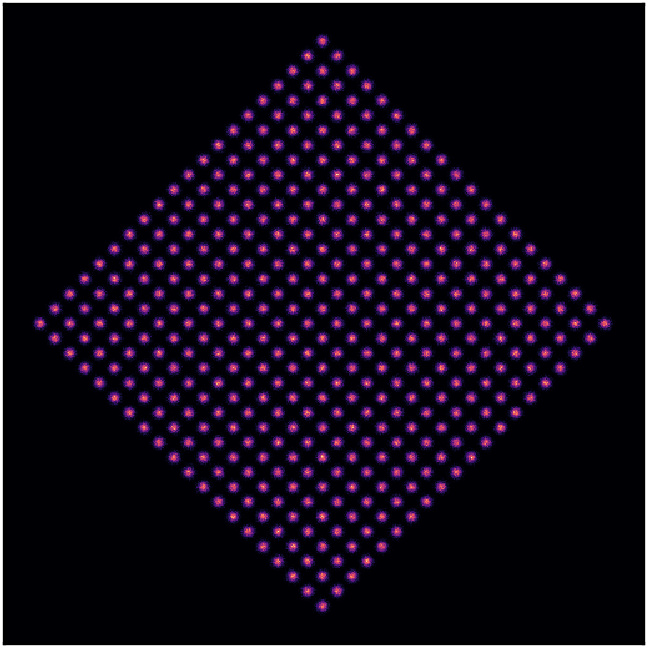
\includegraphics[width=\fw]{figures/synthetic/affine/diamond/diamond-data} &
		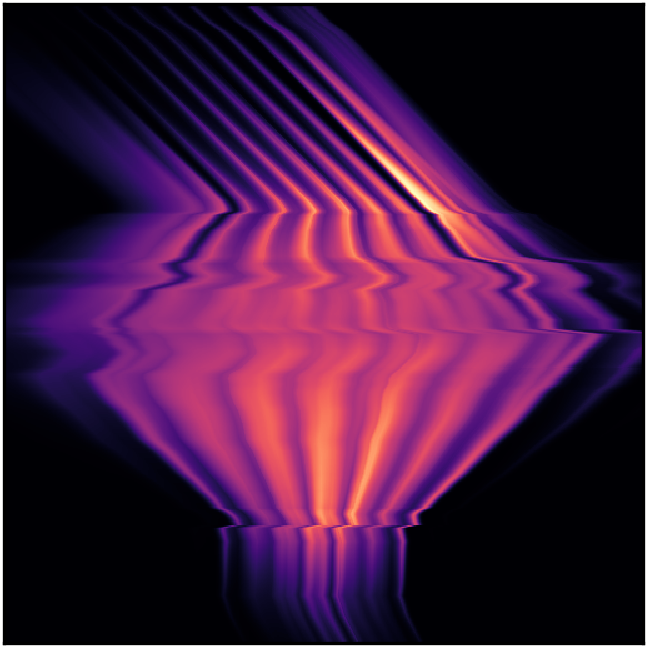
\includegraphics[width=\fw]{figures/synthetic/affine/diamond/diamond-density} &
		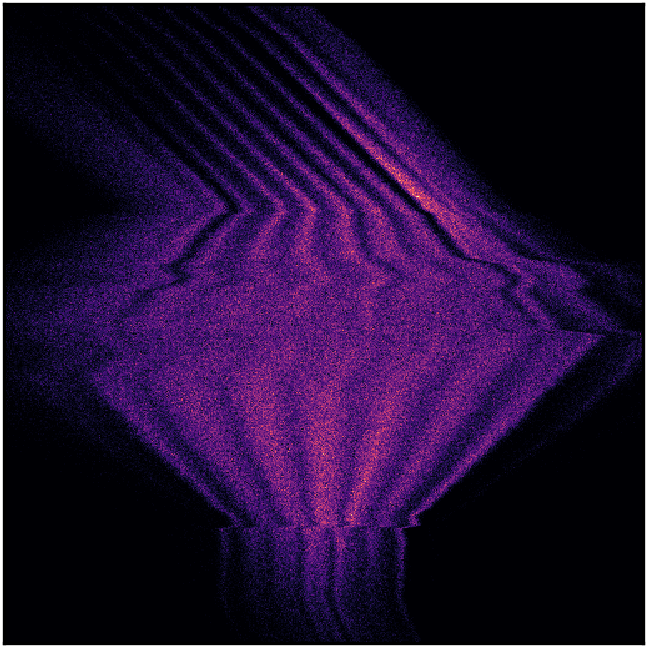
\includegraphics[width=\fw]{figures/synthetic/affine/diamond/diamond-samples} 
		\\
		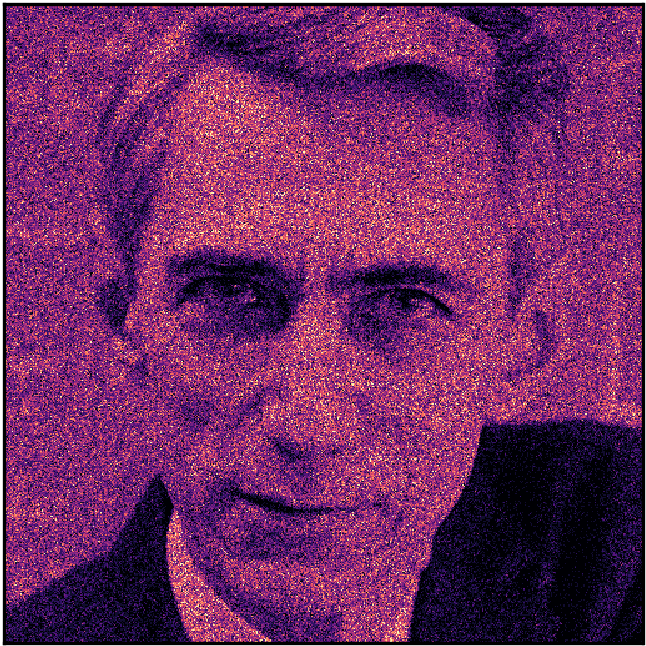
\includegraphics[width=\fw]{figures/synthetic/affine/shannon/shannon-data} &
		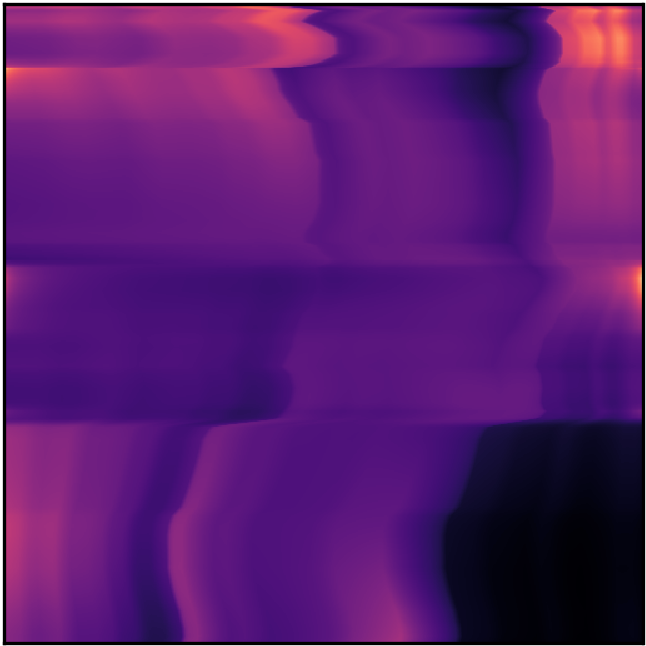
\includegraphics[width=\fw]{figures/synthetic/affine/shannon/shannon-density} &
		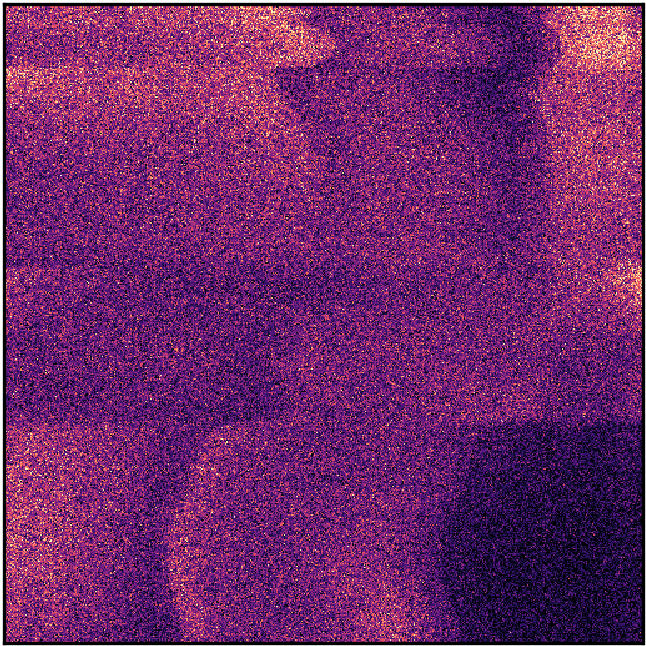
\includegraphics[width=\fw]{figures/synthetic/affine/shannon/shannon-samples}
	\end{tabular}
	\caption{Qualitative results for two-dimensional synthetic datasets using two affine coupling layers.}
	\label{fig:affine-plane-fits}
\end{figure}

\subsection{Samples}

Image samples for VAE experiments are shown in \cref{fig:vae-samples}. Additional samples for generative image-modeling experiments are shown in \cref{fig:image-samples-big}.

\begin{figure}[h!]
	\centering
	\begin{tabular}{cc}
		
\includegraphics[width=\fg]{figures/vae/mnist/mnist-data.png} &
		
\includegraphics[width=\fg]{figures/vae/emnist/emnist-data.png} 
		\\
		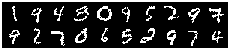
\includegraphics[width=\fg]{figures/vae/mnist/mnist-coupling-data.png} &
		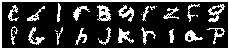
\includegraphics[width=\fg]{figures/vae/emnist/emnist-coupling-data.png} 
		\\
		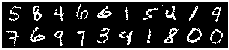
\includegraphics[width=\fg]{figures/vae/mnist/mnist-autoregressive-data.png} &
		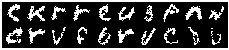
\includegraphics[width=\fg]{figures/vae/emnist/emnist-autoregressive-data.png}
		\\
		(a) MNIST & (b) EMNIST-letters
	\end{tabular}
	\caption{VAE samples. Top to bottom: training data, RQ-NSF (C), RQ-NSF (AR). 
	}
	\label{fig:vae-samples}
\end{figure}

\begin{figure}[h!]
	\centering
	\begin{subfigure}[b]{\fg}
		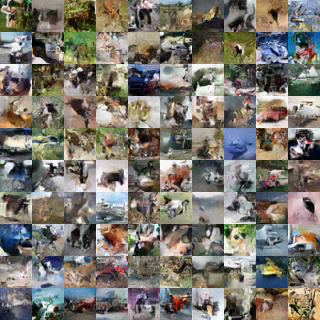
\includegraphics[width=\linewidth]{figures/images/cifar10-5bit-big.png}
		\caption{CIFAR-10 5-bit}
	\end{subfigure}
	\hspace{0.2cm}
	\begin{subfigure}[b]{\fg}
		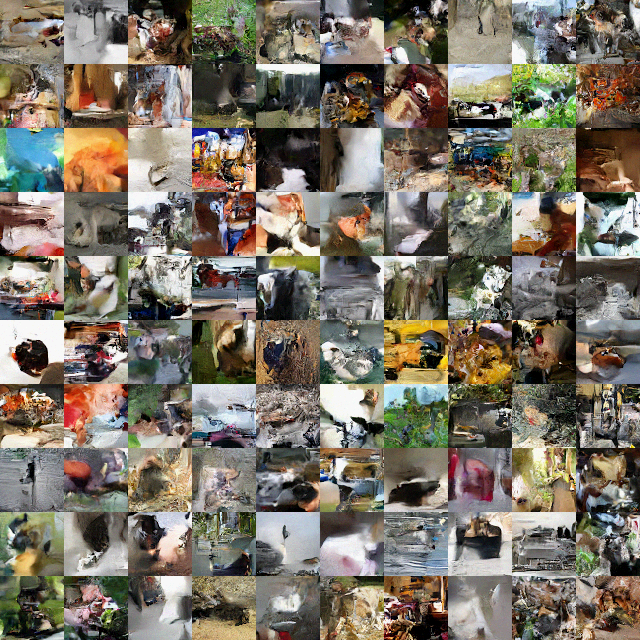
\includegraphics[width=\linewidth]{figures/images/imagenet64-5bit-big.png}
		\caption{ImageNet64 5-bit}
	\end{subfigure}
	\\
	\vspace{0.1cm}
	\begin{subfigure}[b]{\fg}
		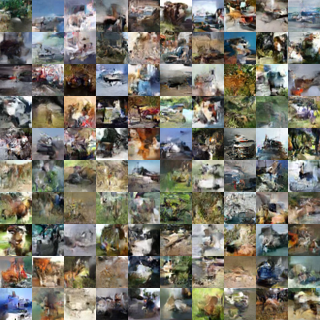
\includegraphics[width=\linewidth]{figures/images/cifar10-8bit-big.png}
		\caption{CIFAR-10 8-bit}
	\end{subfigure}
	\hspace{0.2cm}
	\begin{subfigure}[b]{\fg}
		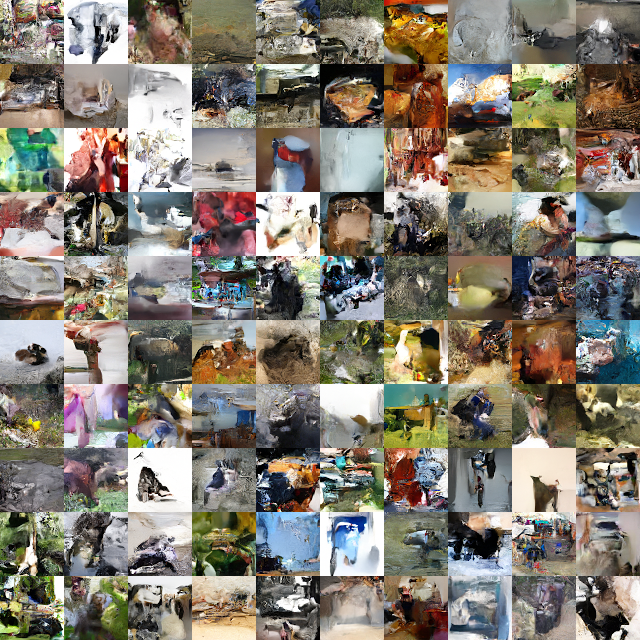
\includegraphics[width=\linewidth]{figures/images/imagenet64-8bit-big.png}
		\caption{ImageNet64 8-bit}
	\end{subfigure}
	\caption{Additional image samples for generative image-modeling experiments.}
	\label{fig:image-samples-big}
\end{figure}
